% =====================================================================
\section{Analysis}
\label{sec:analysis}
% =====================================================================

% ---------------------------------------------------------------------
\subsection{Task 1: Business ecosystem}
\label{sec:t1}
% ---------------------------------------------------------------------

According to \citet[Def.~4.1]{OverbyAudestad2021}, the digital economy ecosystem consists of relationships and dependencies linking digital services, ICT infrastructures, digital markets and authorities within a socioeconomic context. The textbook draws on Moore's original concept of business ecosystems. Nord Pool fits this view because its ecosystem extends across financial markets, electricity grids, ICT and government. The direct and indirect stakeholders are listed in Table~\ref{tab:stakeholders}. Figure~\ref{fig:ecosystem} presents the main dependencies through the textbook's notation for one-way and mutual dependence \citep[Fig.~4.3]{OverbyAudestad2021}.

\begin{table}[ht]
\centering
\small
\caption{Direct and indirect stakeholders in the Nord Pool ecosystem.}
\label{tab:stakeholders}
\begin{tabularx}{\textwidth}{L{3.3cm} L{1.4cm} Y Y}
\toprule
\textbf{Actor} & \textbf{Type} & \textbf{Role} & \textbf{Key dependency} \\
\midrule
Nord Pool AS & Platform & Day-ahead and intraday markets, central counterparty, market data & Needs TSO capacities, members' liquidity, Euronext's capital and technology \\
Euronext (66\%) & Direct & Capital, exchange technology, futures market and clearing house (from 2026) & Earns revenue from Nord Pool; its futures are based on the Nordic system price \\
Statnett, Svenska kraftnät, EPSO-G/Litgrid (34\% via TSO Holding) & Direct & Owners; the TSOs supply cross-zonal capacities and operate grids & Depend on market coupling to allocate capacity \\
Fingrid, Energinet and other coupling TSOs & Direct & Supply capacities; no ownership since 2022 & Essential input without an ownership voice \\
Market participants (about 400 firms) & Direct & Generators, retailers, industrials, traders, aggregators & Need liquidity and guaranteed settlement \\
EPEX SPOT and other NEMOs & Direct & Competitors for members since 2020; partners in SDAC & Coopetition in the shared coupling \\
Regulators (national, ACER, EU) & Direct & NEMO designation, CACM rules, REMIT surveillance, cybersecurity rules & Set the rules of the game \\
Households and firms on spot contracts & Indirect & Pay prices formed on the platform & No influence over the platform \\
Futures traders (Euronext, EEX) & Indirect & Hedge using system-price contracts & Depend on the credibility of the system price \\
Data users & Indirect & Retailers, analysts, researchers, app developers & Depend on access to price data \\
Owner states and Euronext shareholders & Indirect & Owners of the partners & Indirect financial and policy interest \\
\bottomrule
\end{tabularx}
\end{table}

\textbf{Direct stakeholders.} Nord Pool AS runs the day-ahead and intraday markets, serves as central counterparty for all trades and provides market data \citep{NPAbout,NPClearing}. Each alliance partner brings different resources to the platform. Euronext supplies capital, exchange technology and financial distribution, and since March 2026 has also operated a Nordic power futures market and its associated clearing house \citep{Euronext2026}. The TSOs supply an input that no other actor can provide: the cross-zonal transmission capacities needed to calculate area prices. Bids from market participants provide the liquidity. EPEX SPOT has competed for Nordic day-ahead members since entering the market in 2020, while also cooperating in the shared European day-ahead coupling \citep{EPEX2020}. Regulators designate exchanges as nominated electricity market operators (NEMOs), establish coupling rules under the CACM guideline \citep{CACM2015} and oversee market integrity.

\textbf{Indirect stakeholders.} Every auction affects households and firms with spot-price contracts, even though they do not submit bids themselves. Futures traders use the Nordic system price calculated by Nord Pool, which is the reference price for most standard financial contracts in the Nordic region \citep{NPPrice}. Electricity retailers, researchers and other data users purchase or reuse the price data Nord Pool provides \citep{NPData,ERR2022}. Ownership also gives the states behind the TSOs and Euronext's shareholders an indirect stake in the ecosystem.

% Figure 1: Ecosystem map (dependency notation after Øverby & Audestad, Fig. 4.3)
\begin{figure}[ht]
\centering
\begin{tikzpicture}[
  font=\footnotesize,
  box/.style={draw, rounded corners=2pt, align=center, text width=3.3cm, minimum height=1.0cm, fill=white},
  core/.style={box, text width=2.8cm, fill=blue!8, draw=blue!60!black, line width=0.8pt},
  partner/.style={box, fill=orange!10, draw=orange!70!black},
  ind/.style={box, text width=2.5cm, fill=gray!8, draw=gray!60, dashed},
  dep/.style={-{Stealth[length=2.2mm]}, thick},
  mut/.style={{Stealth[length=2.2mm]}-{Stealth[length=2.2mm]}, thick},
  lbl/.style={font=\scriptsize, fill=white, inner sep=1pt, align=center}
]
% core column
\node[core] (np)   at (0,0.9)   {\textbf{Nord Pool AS}\\day-ahead, intraday,\\CCP, data};
\node[box]  (epex) at (0,-1.4)  {\textbf{EPEX SPOT}\\(other NEMOs)};
\node[font=\scriptsize\itshape, text=blue!50!black] (sdaclbl) at (0,-2.3) {SDAC: shared coupling};
\begin{scope}[on background layer]
  \node[draw=blue!50, dashed, rounded corners=4pt, fill=blue!3, inner sep=6pt,
        fit=(np)(epex)(sdaclbl)] (sdac) {};
\end{scope}
\node[box, text width=4.4cm] (reg) at (0,3.5) {\textbf{Regulators}\\NEMO designation, CACM,\\REMIT, NIS2/NCCS};

% left column
\node[partner] (eur) at (-5.5,0.9)  {\textbf{Euronext} (66\%)\\capital, technology,\\futures, clearing};
\node[box]     (mem) at (-5.5,-1.4) {\textbf{Market participants}\\(about 400 firms)};

% right column: all TSOs
\node[partner] (tso)  at (5.5,0.9)  {\textbf{Owner TSOs} (34\%)\\Statnett,\\Svenska kraftnät,\\Litgrid (via EPSO-G)};
\node[box]     (ntso) at (5.5,-1.4) {\textbf{Non-owner TSOs}\\Fingrid, Energinet, \dots};
\begin{scope}[on background layer]
  \node[draw=orange!60!black, dotted, rounded corners=4pt, inner sep=5pt, fit=(tso)(ntso)] (tsos) {};
\end{scope}

% bottom row: indirect stakeholders
\node[ind] (cons) at (-5.5,-4.6) {Households and firms on spot contracts};
\node[ind] (fut)  at (-2.4,-4.6) {Futures traders\\(Euronext, EEX)};
\node[ind] (data) at (2.4,-4.6)  {Data users};
\node[ind] (own)  at (5.5,-4.6)  {Owner states;\\Euronext shareholders};

% dependencies: A -> B means "A depends on B"
\draw[mut] (eur) -- node[lbl, above=2pt]{ownership $\leftrightarrow$\\technology, capital} (np);
\draw[dep] (np.east) -- node[lbl, above=2pt]{capacity data for\\area prices (all TSOs)} (tsos.west |- np.east);
\draw[dep] (ntso) -- node[lbl, above=2pt]{depend on\\coupling} (ntso -| sdac.east);
\draw[mut] (mem) -- node[lbl, above=2pt]{liquidity $\leftrightarrow$\\settlement} (mem -| sdac.west);
\draw[dep] (np) -- node[lbl, right]{designation} (reg);
\draw[dep] (cons) -- node[lbl, right]{price pass-through} (mem);
\draw[dep] (fut.north) -- node[lbl, pos=0.22]{system price} (np.south west);
\draw[dep] (data.north) -- node[lbl, pos=0.22]{price data} (np.south east);
\draw[dep, dotted] (own) -- node[lbl, right]{ownership interest} (tsos.south -| own);
\end{tikzpicture}
\caption{Ecosystem map of the Nord Pool alliance. An arrow from A to B means that A depends on B, and a double arrow means mutual dependence \citep[notation after][Fig.~4.3]{OverbyAudestad2021}. Orange boxes are alliance partners, and dashed boxes are indirect stakeholders. Nord Pool depends on all TSOs for the capacity data behind the area prices, while the TSOs depend on the shared SDAC coupling rather than on Nord Pool specifically.}
\label{fig:ecosystem}
\end{figure}


\textbf{Critical relationships and dependencies.} The most critical relationship is between Nord Pool and the TSOs, and it is asymmetric. The area-price calculation requires the transmission capacities supplied by the TSOs. The Nordic system price is calculated differently: transmission capacities between the Nordic bidding areas are set to infinity, removing internal Nordic congestion restrictions. However, flows between the Nordics and surrounding markets from the area-price calculation enter the system-price calculation as import or export orders \citep{NPPrice}. The system price is therefore not independent of TSO capacity inputs, even though internal Nordic capacity constraints are removed.

The TSOs rely on the overall market coupling, rather than on Nord Pool alone. Since the multi-NEMO arrangement began operating in 2020, capacities have been allocated through a shared coupling that also includes EPEX \citep{EPEX2020}. Price differences between zones generate congestion income for the TSOs \citep{EU2019943}. Nord Pool depends on TSO inputs, while the TSOs depend on the shared coupling rather than exclusively on this particular exchange.

\textbf{Complementarities.} The alliance illustrates the complementarities described by \citet{Jacobides2018}: combining Euronext's commercial and technological capabilities with the TSOs' system knowledge, legitimacy and data increases the value of both partners' contributions. This interpretation follows Appendix~B.1, evaluated against Euronext's acquisition rationale, Nord Pool's price-calculation documentation and Jacobides et al.'s complementarity concept \citep{Euronext2020,NPPrice,Jacobides2018}. The relationship between spot and futures markets provides another example. A liquid spot market gives the system price credibility as a reference, helping support the futures market Euronext launched in March 2026 \citep{Euronext2026}. This reference is also used by a competitor: the underlying for EEX's Nordic system price futures is ``the Nordic Elspot System Price as determined by NordPool'' \citep{EEX2024}. Nord Pool and EPEX also show how cooperation and competition can coexist. They seek the same members but work together on a common price calculation, demonstrating coopetition \citep[Def.~8.4]{OverbyAudestad2021}.

\textbf{How the alliance changes roles, incentives and influence.} Under the alliance, Nord Pool has moved away from being a utility-like exchange owned by grid operators and towards being a commercial platform under the control of a listed group. Euronext explained the acquisition as a way to broaden its revenue, develop Oslo as its Nordic hub and ``reinforce our commodities franchise'' \citep{Euronext2020}. Later developments reflect these commercial aims. In 2022, Nord Pool restricted free access on its website to hourly day-ahead prices from 2021 onwards. Older data became accessible through a paid service in its data portal, which had carried historical data since 2012. Nord Pool attributed the change to rising costs \citep{ERR2022}. Access to licensed price data requires payment from retailers \citep{NPData}. After acquiring Nasdaq's Nordic power futures \citep{FOW2025}, Euronext relaunched them under the name Euronext Nord Pool Power Futures. Trading takes place on Euronext's Optiq platform and clearing on Euronext Clearing, with Nord Pool supplying the underlying system and spot prices \citep{Euronext2026}.

The TSOs still have influence, but they exercise it in a different way. Despite holding 34\% of the shares, they occupy only one of the six shareholder seats on the eight-member board; the other two seats belong to employee representatives. The chair is an Euronext executive, and four other shareholder-side members are listed with job titles but without named employers \citep{NPBoard}. Fingrid and Energinet sold their stakes in TSO Holding in 2022 \citep{EPSOG2022}, but their capacity data remain essential. The TSOs therefore exercise influence mainly through regulation and governance of the shared coupling, rather than through ownership. The resulting governance asymmetry gives those who provide the critical input and bear the system risk limited influence over commercial decisions. This makes regulators more important within the ecosystem, in line with the textbook's account of authorities acting as watchdogs \citep[Sect.~4.7]{OverbyAudestad2021}.

The ecosystem has also continued to change, placing it in a transient rather than a stationary state \citep[Sect.~4.2]{OverbyAudestad2021}. Over six years, the changes have included a new controlling owner (2020), the arrival of a competing exchange (2020), a revised ownership mix in TSO Holding (2022), flow-based capacity calculation (2024; \citealp{NPFlowBased2024}), new products (2025) and a new futures market (2026). Although the core actors remained, their roles were redistributed. Our assessment therefore describes the alliance at one point in time, while the relative influence of Euronext and the TSOs continues to develop.

% ---------------------------------------------------------------------
\subsection{Task 2: Network effects and path dependency}
\label{sec:t2}
% ---------------------------------------------------------------------

A network effect occurs when a user's perceived value of a service changes with the number of users or the amount of usage \citep[Def.~9.1]{OverbyAudestad2021}. The textbook emphasises that this demand-side effect differs from supply-side economies of scale. This distinction matters for Nord Pool. High fixed IT costs and almost no marginal cost per trade mean that an exchange gains a cost advantage from operating at a larger scale; this does not itself constitute a network effect. Table~\ref{tab:ne} summarises the network effects we identify. The five effects follow the list in Appendix~B.2, evaluated using the textbook's network-effect definitions and the sources cited below \citep[Sect.~9.2--9.5]{OverbyAudestad2021}. Their strength ratings are qualitative assessments.

\begin{table}[ht]
\centering
\small
\caption{Network effects associated with the Nord Pool platform.}
\label{tab:ne}
\begin{tabularx}{\textwidth}{L{3.2cm} L{3.4cm} L{2.0cm} Y}
\toprule
\textbf{Effect} & \textbf{Type} & \textbf{Sign, strength} & \textbf{Evidence / mechanism} \\
\midrule
Buyers $\leftrightarrow$ sellers & Cross-side, direct & +, strong & Liquidity: more counterparties give better prices and execution \citep{Pagano1989} \\
Sellers $\leftrightarrow$ sellers & Same-side, direct & $-$, weak & Price competition among sellers; offset by a more robust price \\
Market coupling (zones, TSOs) & Cross-side, indirect; shared by all NEMOs & +, strong & More zones widen the set of feasible trades \citep{Newbery2016} \\
Data accumulation & Data network effect, indirect & +, moderate & More trades produce a richer price history and more valuable data \citep{NPData} \\
Spot $\leftrightarrow$ futures & Cross-market, indirect & +, strong & A credible system price supports futures liquidity, and vice versa \citep{NPPrice,Euronext2026} \\
\bottomrule
\end{tabularx}
\end{table}

\textbf{Buyers and sellers.} The main network effect comes from liquidity. Buyers gain better prices and execution when more sellers participate, while sellers gain the same benefits from additional buyers. This is what the textbook calls a positive, direct, cross-side network effect \citep[Sect.~9.4--9.5]{OverbyAudestad2021}. The tendency for trading to gather in one venue is explained by \citet{Pagano1989}: traders follow other traders because greater liquidity lowers trading costs. Within each side, the effects differ. Additional sellers face stronger competition, producing a weak negative effect similar to that experienced by sellers on eBay \citep[Sect.~10.3]{OverbyAudestad2021}. However, participation by more buyers and sellers also makes the clearing price more robust.

\textbf{Institutions and data sources joining.} Adding bidding zones, interconnectors and TSOs increases value by opening up more possible trades. The integration of European electricity markets produces substantial welfare gains, according to \citet{Newbery2016}. The network behind these gains is part of the Single Day-Ahead Coupling (SDAC), rather than belonging to Nord Pool. All NEMOs use the same algorithm and share one price for each zone. Through EU regulation, the strongest network effect has effectively become a commons available to competing exchanges. Trading activity also builds a more detailed price history. Nord Pool offers data covering almost three decades \citep{NPData}, which gives rise to an indirect data network effect \citep[Sect.~9.3]{OverbyAudestad2021}.

\textbf{Complementary services.} Spot and futures markets reinforce each other. Liquidity in the spot market gives the system price credibility, which attracts futures hedging; the opportunity to hedge then attracts participants to the spot market. Euronext reported transferring 173~TWh of open interest to Euronext Clearing at the March 2026 launch, with 86 participants connected to the market \citep{Euronext2026}. EEX reported 20.41~TWh of gross open interest in July 2026, up from 7.86~TWh in July 2025---a reported increase of 160\% \citep[slide~21]{EEX2026}. These figures concern different dates, and Euronext's launch release does not specify whether its measure uses the same gross basis as EEX's. They indicate a substantial inherited position at Euronext alongside rapid growth at EEX; they do not establish that the futures market is tipping towards one venue.

\textbf{Negative network effects.} Connections between markets allow failures to spread as well as creating value. As the textbook explains, technical problems, interruptions and downtime can produce negative network effects when the departure of some users encourages others to leave \citep[Sect.~9.2]{OverbyAudestad2021}. A failure in one part of a coupled market can separate several zones from the coupling, as the incidents of 2019 and 2021 demonstrate \citep{NPIncident2019,SDAC2021}. With multi-NEMO competition, repeated failures at an exchange could begin this process because members can switch to a competitor without leaving the coupled market. The network effects that support Nord Pool's position therefore also make operational reliability a factor in competition, which we return to in Task~4.

\textbf{Path dependency and switching costs.} A market is path-dependent when its development is shaped by its starting point, network effects and external events, leaving several possible equilibria \citep[Def.~11.2]{OverbyAudestad2021}. Even small advantages early on can lead a market to become locked into a particular outcome, as \citet{Arthur1989} shows. By starting in 1996, Nord Pool gained a first-mover position \citep{NPAbout}, and its system price later became the reference for Nordic financial contracts \citep{NPPrice}. This makes the system price a de facto standard \citep[Def.~15.1]{OverbyAudestad2021}: the more contracts that use it, the more expensive it becomes to adopt another reference. Two other mechanisms support this development. \emph{Sunk costs} arise because members have invested in IT and API integration with Nord Pool's trading systems and in collateral arrangements with its clearing function; these investments cannot be recovered if they move to another exchange. \emph{Learning effects} arise because traders and back-office staff already know Nord Pool's order types, interfaces and procedures, so using the incumbent costs less than learning to use a new venue at the same fees. Alongside access to historical data, these mechanisms create switching costs \citep[Def.~12.2]{OverbyAudestad2021}, corresponding to the textbook's categories of investments and training \citep[Sect.~12.3]{OverbyAudestad2021}.

\textbf{Lock-in, tipping and winner-takes-all.} Before 2020, the Nordic spot market had effectively tipped in Nord Pool's favour. Regulation has since aimed to make switching between exchanges less costly. Under CACM, several NEMOs can operate in the same country, and the Nordic multi-NEMO arrangement began operating on 3~June 2020 \citep{EPEX2020,CACM2015}. Common products, including the 15-minute products introduced in SDAC from 1~October 2025 \citep{OTE2025}, make exchanges more interchangeable. The comparison in the textbook is number portability: regulation reduces lock-in by making it easier to move between providers \citep[Sect.~12.6]{OverbyAudestad2021}. EPEX's 54~TWh of Nordic day-ahead trading in 2024 shows that it has gained a foothold, rather than taken over the market \citep{EPEX2025}. We therefore describe the spot market as one in which the incumbent can be challenged, rather than as a winner-takes-all monopoly. Nord Pool charges €0.040/MWh for day-ahead trading \citep{NPFees2026}. Competition may help keep this fee low, but the available evidence does not show why the fee is set at this level.

Lock-in remains, but its source may be changing. The system price, historical data and futures market are held within the Euronext group and face less competition from the multi-NEMO arrangement than the auction does. Viewed through the lock-in cycle \citep[Sect.~12.4]{OverbyAudestad2021}, integrating spot and futures activities can strengthen the dependence of participants who use both markets for trading and hedging.

% ---------------------------------------------------------------------
\subsection{Task 3: Multisided platform mapping}
\label{sec:t3}
% ---------------------------------------------------------------------

\textbf{Is Nord Pool a multisided platform?} An MSP allows two or more distinct user groups, each affiliated with the platform, to interact directly \citep[Def.~10.1]{OverbyAudestad2021}, building on \citet{HagiuWright2015}. Nord Pool raises a classification problem. It acts as central counterparty for trades \citep{NPClearing}, meaning that it formally buys from sellers and sells to buyers. This resembles the textbook's reseller, which is distinguished from an MSP \citep[Sect.~10.5]{OverbyAudestad2021}. The difference is that participants choose their bid prices and quantities, while Nord Pool handles matching and settlement instead of purchasing electricity under its own resale strategy. Trading is also anonymous, so buyers and sellers never meet. We therefore read direct interaction as \citet{HagiuWright2015} define it: the sides keep control over the key terms of the trade, rather than meeting in person. On this basis, we classify the trading service as an MSP and central clearing as an additional risk-management service.

\textbf{The sides and the platform boundary.} We identify two core trading sides (Figure~\ref{fig:msp}):
\begin{enumerate}
  \item Sellers: generators and other participants offering electricity.
  \item Buyers: retailers, industrial consumers and other participants purchasing electricity.
\end{enumerate}
The same firm can buy electricity in one period and sell it in another. We therefore define the sides by what participants do in a trade.

Small participants and aggregators participate as buyers or sellers. The Small Participant tariff is a pricing segment within these sides, not a separate side merely because its fees differ. Data customers buy an ancillary service derived from trading activity. We do not treat them as a separate core trading side, since buying price data does not by itself demonstrate direct interaction with another affiliated group. Futures traders participate in complementary markets operated by Euronext or EEX. They depend on Nord Pool's reference prices but are not, on that basis alone, a side of Nord Pool's physical trading platform. TSOs are partners supplying a critical input. Households on retail spot-price contracts are indirect stakeholders rather than affiliated platform users.

\textbf{Competition.} The textbook distinguishes three forms of competition involving MSPs \citep[Sect.~10.2.3]{OverbyAudestad2021}. First, Nord Pool competes directly with EPEX SPOT for trading members. Second, alternative services compete for particular customer needs: bilateral contracts compete for trading volume, and free data from the ENTSO-E Transparency Platform provides an alternative for some data users. Third, competition occurs among users on the same side, such as generators submitting electricity offers to the auction. Together, these forms restrict the platform's freedom to set prices and make commercial decisions.

\textbf{Strength of the network effects.} The buyer--seller effect is positive in both directions: additional counterparties can improve trading opportunities and liquidity. Competition between sellers can create a negative same-side effect, although broader participation also supports price formation. Small participants contribute through their buyer or seller role, rather than creating a separate cross-side effect simply because they use another tariff. Trading activity also creates valuable information for data customers, and the reference price supports complementary futures markets. These are relationships across services and markets, distinct from the core buyer--seller interaction.

% Figure 2: Multisided platform map with network effects and prices
\begin{figure}[ht]
\centering
\begin{tikzpicture}[
  font=\footnotesize,
  side/.style={draw, rounded corners=2pt, align=center, text width=3.1cm, minimum height=1.25cm, fill=green!6, draw=green!40!black},
  plat/.style={draw, rounded corners=3pt, align=center, text width=3.6cm, minimum height=1.6cm, fill=blue!8, draw=blue!60!black, line width=0.8pt},
  partner/.style={draw, rounded corners=2pt, align=center, text width=3.8cm, minimum height=1.1cm, fill=orange!10, draw=orange!70!black, dashed},
  aff/.style={thick, gray!70},
  ne/.style={{Stealth[length=2mm]}-{Stealth[length=2mm]}, thick, red!65!black},
  ne1/.style={-{Stealth[length=2mm]}, thick, red!65!black},
  lbl/.style={font=\scriptsize, fill=white, inner sep=1pt, align=center}
]
\node[plat] (np) at (0,0) {\textbf{Nord Pool}\\matching, system price,\\central clearing};
\node[side] (sel) at (-4.8,0.9)  {\textbf{Sellers}\\(generators)\\\scriptsize €21.5k/yr + €0.055/MWh};
\node[side] (buy) at (4.8,0.9)   {\textbf{Buyers}\\(retailers, industrials)\\\scriptsize €21.5k/yr + €0.055/MWh};
\node[side] (sml) at (-4.8,-2.3) {\textbf{Small participants,}\\\textbf{aggregators}\\\scriptsize €0/yr + €0.140/MWh};
\node[side] (dat) at (4.8,-2.3)  {\textbf{Data customers}\\\scriptsize €600--3,500/yr};
\node[side] (fut) at (0,4.6)   {\textbf{Futures traders}\\(Euronext, EEX)\\\scriptsize pay Euronext/EEX, not Nord Pool};
\node[partner] (tso) at (0,-3.2) {\textbf{TSOs} (partner, input)\\capacity data; no trading fee};

% affiliation lines
\foreach \s in {sel,buy,sml,dat} \draw[aff] (\s) -- (np);
\draw[aff, dashed] (fut) -- node[lbl]{system price} (np);
\draw[aff, dashed, orange!70!black] (tso) -- node[lbl]{capacities} (np);

% network effects
\draw[ne] (sel.north) to[out=25,in=155] node[lbl, pos=0.5, yshift=1pt]{(+/+) strong cross-side} (buy.north);
\draw[ne] (sml.north) -- node[lbl, right]{(+/+) moderate:\\depth, flexibility} (sel.south);
\draw[ne1] (buy.south) -- node[lbl, right]{traders $\rightarrow$ data\\(+/0) one-way} (dat.north);
\draw[ne, red!50] (sel.west) to[out=150,in=210, looseness=5] node[lbl, left]{($-$/$-$)\\same-side} (sel.south west);
\end{tikzpicture}
\caption{Nord Pool as a multisided platform. Grey lines show affiliation with the platform, and red arrows show network effects with SRM-style signs. Prices are day-ahead fees from the 2026 fee schedule (trading + clearing) and data prices \citep{NPFees2026,ERR2022,NPData}. Buyers and sellers pay identical fees. TSOs are partners supplying an input, not a paying side, and consumers are not affiliated with the platform.}
\label{fig:msp}
\end{figure}


\textbf{Pricing.} Nord Pool publishes its trading fees, allowing us to analyse actual pricing rather than invent a pricing architecture (Table~\ref{tab:pricing}). Standard participants pay an annual fee of €21,500 for day-ahead and intraday continuous access, plus €0.040/MWh for day-ahead trading and €0.015/MWh for clearing \citep{NPFees2026}. The published tariff does not differentiate between the buyer and seller roles. There is therefore no free trading side. Buyers and sellers pay the same fees, even though they may respond differently to price changes.

\begin{table}[ht]
\centering
\small
\caption{Nord Pool's trading tariffs and related service prices, with MSP interpretation. Sources: \citet{NPFees2026}, \citet{ERR2022}, \citet{NPData}.}
\label{tab:pricing}
\begin{tabularx}{\textwidth}{L{3.0cm} L{5.4cm} Y}
\toprule
\textbf{Side / segment / actor} & \textbf{Price} & \textbf{Interpretation} \\
\midrule
Buyers and sellers & €21,500/yr + €0.040/MWh trading + €0.015/MWh clearing (day-ahead); intraday continuous €0.109/MWh + €0.015/MWh & Same tariff for both core trading sides \\
Small participants & €0 fixed; day-ahead €0.125/MWh + €0.015/MWh; €3,000/yr floor & Lower entry barrier through a tariff option within the trading sides \\
Largest members & Caps: fixed fees €65,000/yr; clearing €375,000 per member and country; gross volume trading fee €150,000/yr & Fee caps reduce average charges at high activity levels \\
Data customers & Historical access reported at €600/yr in 2022; retailer licence €3,500/yr (restricted publication) & Ancillary service priced separately from trading \\
TSOs & No trading fees in their capacity-provider role; receive congestion income & Infrastructure partners rather than a trading side \\
\bottomrule
\end{tabularx}
\end{table}

Within this structure, different tariff options can encourage participation. The Small Participant option removes the fixed access fee but applies higher variable fees and a €3,000 annual floor for day-ahead trading \citep{NPFees2026}. Members can thus choose between a fixed-plus-usage tariff and a usage-only tariff, one of the combinations of fixed and per-use charges the textbook describes for MSPs \citep[Sect.~10.2.2]{OverbyAudestad2021}. We interpret this as second-degree price discrimination that lowers the entry barrier for smaller members. Larger members benefit from fee caps. Both features can be understood through platform pricing theory: a platform may encourage participation that creates benefits for other users \citep{RochetTirole2003,Armstrong2006}. The tariff alone does not establish the size of any cross-subsidy or show which segment finances another. Our assumption is therefore that small participants and the largest members are subsidised, while mid-sized members using the standard tariff form the net paying segment. This assumption follows from the fee structure: smaller members avoid the fixed fee and the largest members benefit from caps, whereas mid-sized members pay the full fixed fee without reaching a cap.

Data services have separate prices. A 2022 source reported historical-data access at €600 per year for up to three users \citep{ERR2022}. We treat this as a historical observation rather than a verified 2026 price. The electricity-retailer licence is advertised at €3,500 per year and does not permit unrestricted public publication \citep{NPData}. Free data alternatives may constrain willingness to pay, but differences in access, delivery and licence terms mean that the services need not be identical.

Providing capacity does not require TSOs to pay trading fees, although CACM makes TSOs and NEMOs jointly responsible for coupling costs \citep{CACM2015}. They receive congestion income through the coupled market \citep{EU2019943}. Finally, the standard variable day-ahead fee of €0.055/MWh is about 0.15\% of the 2024 average system price (calculated from \citealp{NPFees2026} and \citealp{NP2024}; see Appendix~A.3). Fixed fees are excluded from this comparison, which shows the scale of the charge rather than each member's total trading cost.
% ---------------------------------------------------------------------
\subsection{Task 4: Cybersecurity economics}
\label{sec:t4}
% ---------------------------------------------------------------------

No single firm purchases all the security needed for Nord Pool. Instead, partners protect the parts of the attack surface they control, cover their own protection costs and bear only some of the losses from a failure. We therefore follow \citet{Kianpour2022} in treating platform security as a good that the alliance provides jointly.

\textbf{Provision structure.} The weakest contribution, the sum of contributions or the strongest contribution can determine the level of a public good, as distinguished by \citet{Hirshleifer1983}. All three forms apply to Nord Pool's security. \emph{Best-shot} provision describes the core matching and clearing engine most closely, since protecting this one system protects everyone. Responsibility for operating it rests with Nord Pool. We assume that Euronext's group-level security capabilities support it, but public sources do not explain the integration between the two organisations' security systems, and the hosting location is not stated in the public record.

The interfaces follow \emph{weakest-link} provision. Every NEMO and TSO must submit its inputs on time for European day-ahead coupling to function, and technical problems have repeatedly caused parts of the market to leave the common coupling. On 7~June 2019, EPEX's CWE and GB markets and OMIE were decoupled \citep{NPIncident2019}. On 13~January 2021, Italy and, as a result, Greece, Slovenia and Croatia were decoupled \citep{SDAC2021}. About 400 member firms also connect through systems and credentials of their own \citep{NP2024}, while incorrect or manipulated capacity data from one TSO would affect prices in many zones. Market surveillance and incident response are closer to \emph{total-effort} provision because each partner's effort contributes to detection.

Responsibility for the attack surface is divided among the partners. Group IT and the futures trading and clearing systems fall under Euronext's control \citep{Euronext2026}. Nord Pool manages the trading platform, central counterparty and collateral systems, together with the data portal and APIs. Capacity calculation and grid operational technology are controlled by the TSOs. Members are responsible for their own trading systems and credentials.

\textbf{Who invests and who loses.} The stakeholders from Task~1 are used in Table~\ref{tab:cyber} to map security costs and losses qualitatively. All levels are illustrative assumptions; we do not use probabilities because none are publicly disclosed.

\begin{table}[ht]
\centering
\small
\caption{Cost and loss map for platform security (qualitative; illustrative assumptions, no probabilities).}
\label{tab:cyber}
\setlength{\tabcolsep}{4pt}
\begin{tabularx}{\textwidth}{L{2.2cm} L{1.5cm} L{2.8cm} L{1.9cm} L{1.9cm} Y}
\toprule
\textbf{Actor} & \textbf{Security effort borne (H/M/L)} & \textbf{Loss if breached, $D_i$} & \textbf{Type of loss} & \textbf{Control over the risk} & \textbf{Asymmetry} \\
\midrule
Partner A: Euronext & H (group level) & M: small business line, but reputational spillover to all Euronext markets & Financial, reputational, regulatory & High over group IT; indirect over Nord Pool & Controls much, bears a small share of total loss \\
Platform: Nord Pool AS & H & H: NEMO designation, losses as central counterparty, member trust & Operational, financial, licence & High over platform; none over TSO data & Close to balanced \\
Partner B: owner TSOs (Statnett, SvK; Litgrid via EPSO-G) & M for platform (H for grid) & H: system security, wrong flows, redispatch costs & Physical, operational, social & High over capacity data; low over exchange IT & Loss exceeds their 34\% share and one board seat \\
Non-owner TSOs (e.g.\ Fingrid, Energinet) & M & M--H & Physical, operational & Capacity data only & No ownership voice at all \\
Client institution (e.g.\ a power retailer) & L--M & H: wrong prices, failed settlement, collateral calls & Financial & Own credentials only & Exposed, little control \\
End users / society & None & H: households on spot contracts, security of supply, trust & Financial, social & None & Full asymmetry: no investment decision \\
\bottomrule
\end{tabularx}
\end{table}

\textbf{Incentive asymmetry.} Partners base their investment on their own expected loss, $D_i$, but actual losses extend to client institutions, consumers and society, who have no role in the investment decision. For Euronext, Nord Pool is a small business line: it had about €40 million in revenue in 2018, shortly before the acquisition \citep{Euronext2020}. The group's privately optimal investment level therefore depends on its own revenue and reputation, rather than on the social cost of disruption to the Nordic power market. Together, these privately optimal levels fall below the socially efficient level. \citet{AndersonMoore2006} explain this security externality through misaligned incentives rather than technological weaknesses, and \citet{Kianpour2021} identify it as a central theme in cybersecurity economics.

Network effects from Task~2 make the asymmetry greater. European market coupling allows a failure to spread across zones, and the use of the system price in Nordic financial contracts carries its effects into derivatives. A larger network therefore brings greater losses. The pricing analysis in Task~3 provides another connection. The Small Participant tariff may encourage smaller firms to join by removing the fixed access fee, although a minimum annual charge remains. We assume that some additional members could have fewer security resources, creating further weak entry points. The sources used here do not establish how many members use this tariff, whether it increases participation, or whether these members have weaker security. The connection between the pricing incentive and weakest-link risk is therefore a proposed mechanism rather than an observed outcome.

\textbf{What corrects the asymmetry?} The main response comes from regulation. Nominated electricity market operators are explicitly listed as energy-sector entities under the NIS2 Directive \citep{NIS2}. Under the Network Code on Cybersecurity for electricity, entities that national authorities designate as high- or critical-impact, potentially including market operators, must assess risks and apply minimum or advanced controls \citep{NCCS2024}. Norway's Digital Security Act came into force on 1~October 2025. It implements NIS1 in sectors that include energy and financial market infrastructure \citep{Regjeringen2025}. Financial-market regulation covers futures and clearing activities, which places the alliance under two security regimes. Within market coupling, shared fallback procedures establish joint duties for incident response \citep{NPIncident2019,SDAC2021}, while members' collateral requirements \citep{NPClearing} place settlement risk back with the party that controls it. The public record is silent on service-level agreements \citep[Def.~17.2]{OverbyAudestad2021} between the partners, liability clauses, cyber insurance and security certification requirements; there is therefore no basis for assessing these instruments.

We propose two measures to address weakest-link risks. First, membership terms could set minimum security requirements, supported by fee incentives. Second, TSOs could take part in joint decisions about platform security, since they bear some of the losses from failures. The sources reviewed do not show whether the alliance already uses these measures.

Domestic hosting alone would not resolve the interface and credential risks identified above. Hosting arrangements can affect resilience and the jurisdiction governing access to data, but the sources used here do not identify Nord Pool's hosting provider or locations. Euronext's EU headquarters alone cannot establish where data are stored or which access laws apply. This argument follows Appendix~B.4 and is evaluated using the provision framework and incident evidence discussed above.

% ---------------------------------------------------------------------
\subsection{Task 5: Business model structure}
\label{sec:t5}
% ---------------------------------------------------------------------

The full Business Model Canvas for Nord Pool as an alliance platform is shown in Figure~\ref{fig:bmc} \citep[Sect.~19.2]{OverbyAudestad2021}. In the textbook's classification, Nord Pool represents a value network because it connects members of a market \citep[Def.~8.3]{OverbyAudestad2021}, rather than a value chain. Our analysis covers the four blocks that the alliance has affected most.

\textbf{Key partners.} Listing Euronext and the TSOs as owners would be the conventional approach in a canvas. However, our analysis separates the role of partner from that of owner. Every TSO involved in coupling is a key partner through its supply of capacity data, but direct ownership is limited to Statnett and Svenska kraftnät, Litgrid is represented by its parent group EPSO-G, and Fingrid and Energinet left in 2022 \citep{EPSOG2022}. The futures platform and clearing house also give Euronext a wider partnership role \citep{Euronext2026}. Other NEMOs combine cooperation in the coupling with competition for members.

\textbf{Key resources.} A particularly valuable resource is the reference status of the Nordic system price \citep{NPPrice}. It is based on aggregated orders with internal Nordic transmission capacities set to infinity, but also incorporates import and export flows from the coupled area-price calculation. Its credibility therefore rests on market participation, the price-calculation process and the wider coupled-market infrastructure. The area prices combine participants' orders with the TSOs' capacity inputs in the shared coupling. Nord Pool calculates the system price and publishes price results, while Euronext controls the company through its majority ownership. Other key resources are NEMO designations in 16 countries \citep{NP2024}, almost three decades of price data \citep{NPData}, and members' trust in the clearing guarantee.

\textbf{Revenue streams.} The value of the electricity traded is much greater than the trading and clearing fees collected (Section~\ref{sec:t3}). Data licences are an ancillary revenue stream, but the cited sources do not establish when they were introduced or how their contribution to revenue has changed \citep{ERR2022,NPData}. Euronext's Optiq platform handles trading in the new futures and Euronext Clearing handles their clearing, while ``Nord Pool provides the underlying system and spot prices'' \citep{Euronext2026}. The futures revenue split between Euronext and Nord Pool is not public, leaving the amount recorded in Nord Pool's revenue streams unknown. The alliance offers services that monetise the auction's outputs, but the available figures do not establish a shift in the revenue mix.

\textbf{Value proposition.} For traders, the benefits are liquid, neutral price formation and guaranteed settlement. TSOs benefit from efficient congestion management, while society gains a transparent reference price. This value proposition follows Appendix~B.5, evaluated against Nord Pool's descriptions of its markets and clearing services \citep{NPAbout,NPClearing}. Selling the data creates a tension between the price's role as a public signal and its role as a product.

\textbf{What the canvas reveals about the alliance.} Looking at who contributes to each of the four blocks and who captures its value helps explain how the alliance works. The textbook places key partners and key resources among its four value generation blocks, together with key activities and cost structure. In both blocks, many actors contribute, but the resources are held by a company that Euronext controls through majority ownership. The TSOs provide a key input---the capacity data behind area prices---but receive none of Nord Pool's revenue streams. Their compensation comes through congestion income in the coupling and is therefore outside Nord Pool's canvas \citep{EU2019943}. Treating user groups as separate segments can hide the interactions between them, a problem highlighted by the textbook \citep[Sect.~10.2.4]{OverbyAudestad2021}. For an alliance, a similar risk arises when the canvas treats the partners as a single firm. The canvas becomes useful only when contributions and value capture are assigned to each partner. Charging for price data creates tension with the value proposition of a transparent reference price. The available sources do not show whether data revenue is increasing.

% Figure 3: Business Model Canvas, built in the course template
% (Template_Business Model Canvas.pptx, filled and exported to PDF:
%  Images/bmc_nordpool.pptx -> Images/bmc_nordpool.pdf)
\begin{sidewaysfigure}
\centering
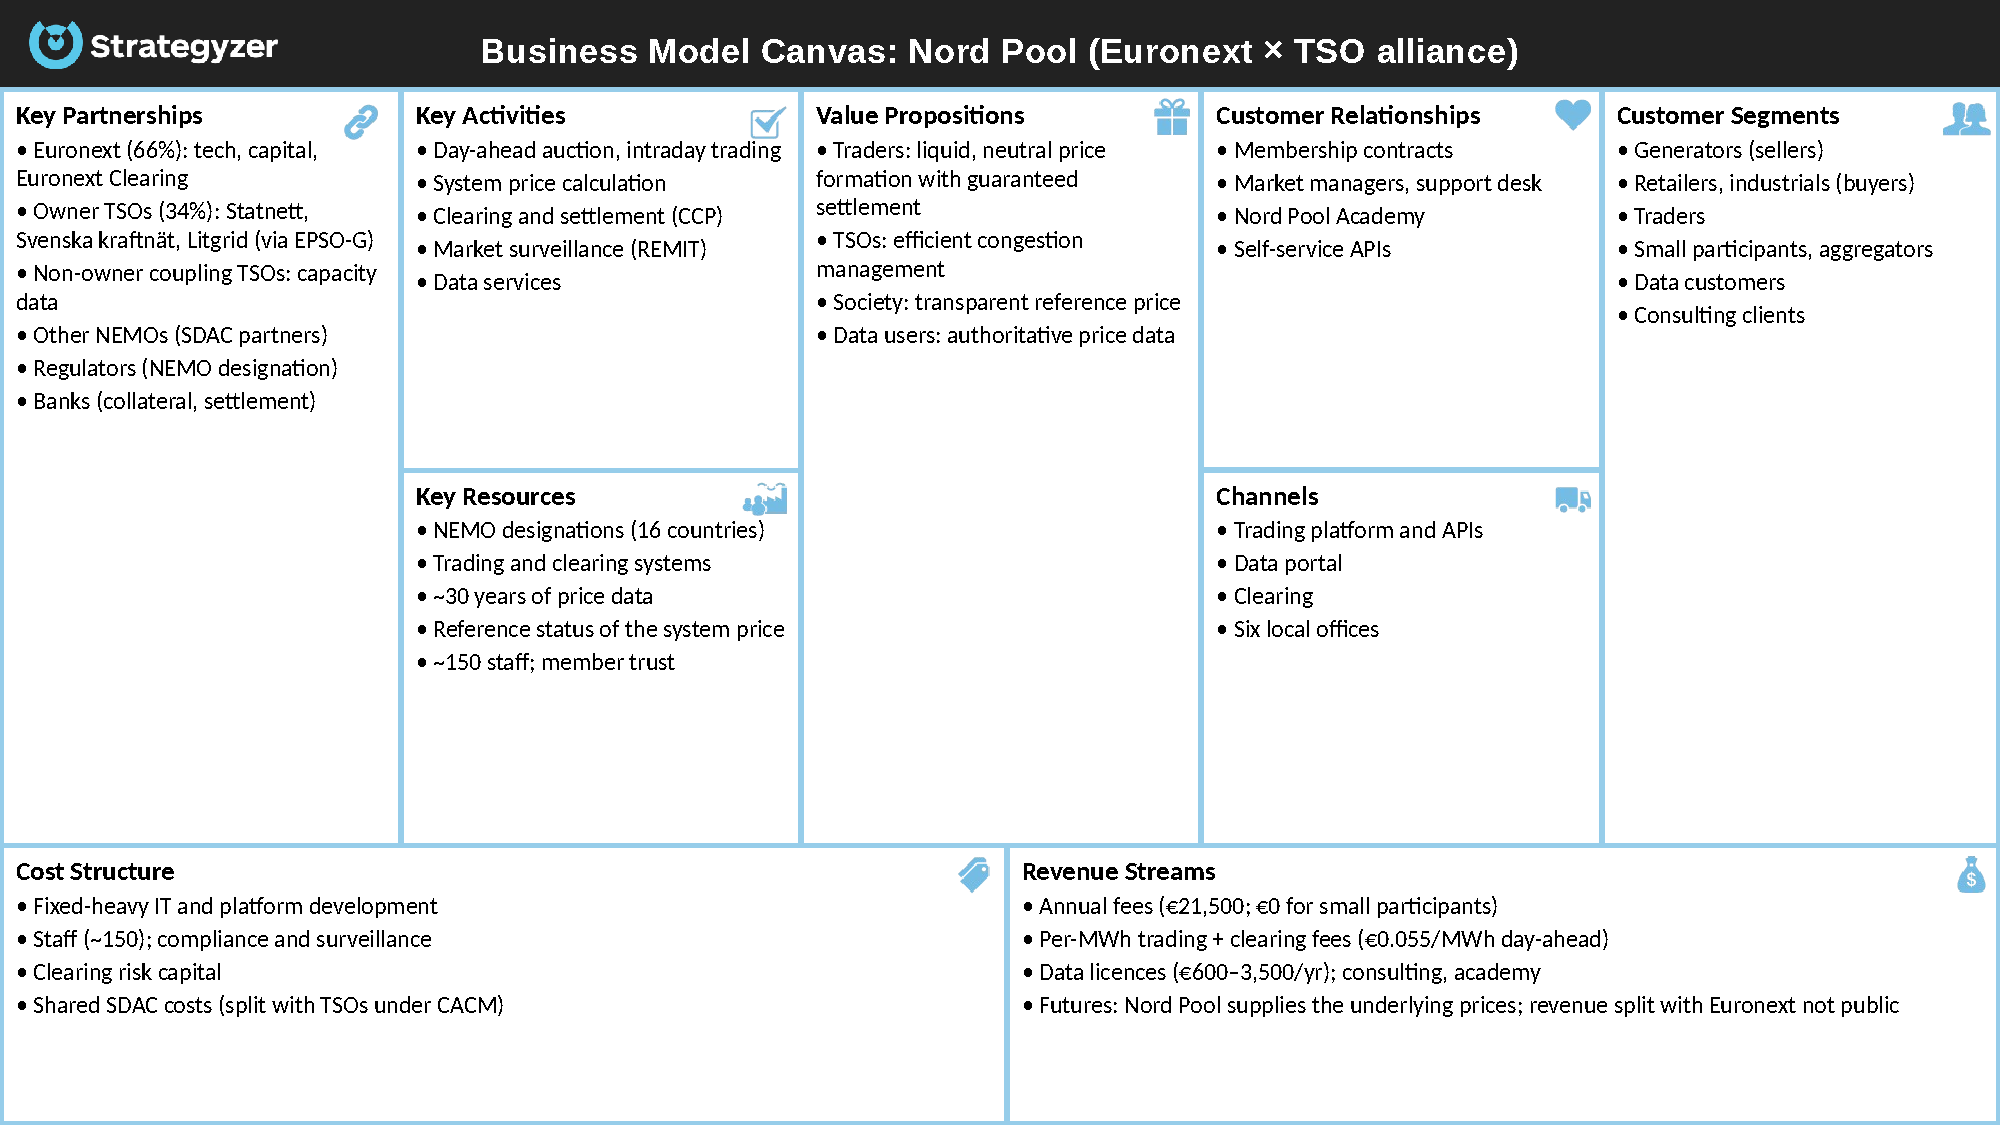
\includegraphics[width=\textheight]{Images/bmc_nordpool.pdf}
\caption{Business Model Canvas for Nord Pool as an alliance platform, made in the course template \citep[building blocks after][Table~19.1]{OverbyAudestad2021}. Prices are from \citet{NPFees2026} and \citet{NPData}; the historical-data price is a 2022 figure \citep{ERR2022}. Staff, offices and countries are from \citet{NPAbout}.}
\label{fig:bmc}
\end{sidewaysfigure}


\textbf{Stakeholder Relationship Model.} Figure~\ref{fig:srm} uses the SRM to add relationships and network effects to the information in the canvas \citep[Sect.~19.3]{OverbyAudestad2021}. These include ownership (66/34), TSO capacity data supplied to Nord Pool, fees and licences, the agreement linking other NEMOs to the coupling, and regulators' NEMO designation. Buyers and sellers have a positive network effect on each other (+/+), as do spot and futures liquidity (+/+), while sellers have a negative same-side effect on each other ($-$/$-$). The benefit that traders create for data users goes in one direction only. Since the textbook provides no notation for this relationship, we use (+/0). The SRM therefore makes visible a dependency that the canvas misses: important relationships involve actors outside Nord Pool's customer segments.

% Figure 4: Stakeholder Relationship Model (notation after Øverby & Audestad, Fig. 19.3)
\begin{figure}[ht]
\centering
\begin{tikzpicture}[
  font=\footnotesize,
  st/.style={draw, rounded corners=2pt, align=center, text width=2.6cm, minimum height=0.9cm, fill=white},
  org/.style={st, fill=blue!8, draw=blue!60!black, line width=0.8pt},
  grp/.style={st, double, double distance=1.2pt},
  rel/.style={-{Stealth[length=2mm]}, thick, gray!65!black},
  rel2/.style={{Stealth[length=2mm]}-{Stealth[length=2mm]}, thick, gray!65!black},
  ne/.style={{Stealth[length=2mm]}-{Stealth[length=2mm]}, thick, red!65!black},
  ne1/.style={-{Stealth[length=2mm]}, thick, red!65!black},
  lbl/.style={font=\scriptsize, fill=white, inner sep=1pt, align=center}
]
% top row
\node[st]  (eur)  at (-5.0,3.0) {Euronext};
\node[st]  (reg)  at (-1.8,3.0) {Regulators};
\node[st]  (tsoh) at (1.8,3.0)  {Owner TSOs\\(TSO Holding)};
\node[grp] (ntso) at (5.0,3.0)  {Non-owner TSOs};
% middle row
\node[grp] (epex) at (-5.0,0.2) {EPEX SPOT /\\other NEMOs};
\node[org] (np)   at (0,0.2)    {\textbf{Nord Pool}};
\node[grp] (dat)  at (5.0,0.2)  {Data customers};
% member row
\node[grp] (sel)  at (-3.0,-2.2) {Sellers};
\node[grp] (buy)  at (3.0,-2.2)  {Buyers};
% bottom row
\node[grp] (sml)  at (-5.2,-4.3) {Small participants};
\node[grp] (cons) at (0.6,-4.3)  {Consumers};
\node[grp] (fut)  at (5.2,-4.3)  {Futures traders};

% relationships
\draw[rel]  (eur.south)  -- node[lbl, pos=0.3, below left=1pt]{66\% ownership} (np.north west);
\draw[rel]  (reg.south)  -- node[lbl, pos=0.4, left=2pt]{designation,\\supervision} (np.north);
\draw[rel]  (tsoh.south) -- node[lbl, pos=0.4, left=2pt]{34\% ownership,\\capacity data} (np.north east);
\draw[rel]  (ntso.south west) -- node[lbl, pos=0.3, below right=1pt]{capacity data} (np.east);
\draw[rel2] (epex) -- node[lbl, above=2pt]{SDAC agreement;\\competition} (np);
\draw[rel]  (dat) -- node[lbl, below=2pt]{licence fees} (np);
\draw[rel]  (sel.north east) -- node[lbl, left=3pt]{fees, collateral} (np.south west);
\draw[rel]  (buy.north west) -- node[lbl, right=3pt]{fees, collateral} (np.south east);
\draw[rel]  (cons) -- node[lbl, right=2pt]{retail contracts} (buy.south west);

% network effects
\draw[ne]  (sel) -- node[lbl]{(+/+)} (buy);
\draw[ne]  (sml) -- node[lbl, left=2pt]{(+/+)} (sel);
\draw[ne1] (buy.north east) -- node[lbl, right=2pt]{(+/0)} (dat.south);
\draw[ne]  (fut) -- node[lbl, right=2pt]{(+/+) spot--futures\\liquidity} (buy.south east);
\draw[ne, red!50] (sel.north west) to[out=150,in=210, looseness=6] node[lbl, left]{($-$/$-$)} (sel.south west);
\end{tikzpicture}
\caption{Stakeholder Relationship Model. Double-bordered boxes are groups of similar stakeholders. Grey arrows show relationships (asset exchange, formal agreements), and red arrows show network effects using the SRM notation of \citet[Sect.~19.3]{OverbyAudestad2021}. The one-way effect of traders on data customers, (+/0), extends the textbook notation.}
\label{fig:srm}
\end{figure}

